 %%
%% Created in 2018 by Martin Slapak
%%
%% Based on file for NRP report LaTeX class by Vit Zyka (2008)
%%
%% Compilation:
%% >pdflatex report
%% >bibtex report
%% >pdflatex report
%% >pdflatex report

\documentclass[czech]{mvi-report}

\usepackage[utf8]{inputenc}
\usepackage{amsmath}
\usepackage{colortbl}
\usepackage{listings}
\usepackage{bm}

\usepackage{graphicx}
\graphicspath{ {./img/} }

\title{DÚ č.3 - Markovské řetězce s diskrétním časem}

\author{Marek Nevole, Jan Novotný}
\affiliation{ČVUT - FIT}
\email{\{nevolmar, novot103\}@fit.cvut.cz}

\def\file#1{{\tt#1}}

\begin{document}

\maketitle

%%%%%%%%%%%%%%%%%%%%%%%%%%%%%%%%%%%%%%%%%%%%%%%%%%%%%%%%%%%%%%%%%%%%%%%%%%%%%%%%
\section{Úvod}
Ve třetím úkolu z předmětu vybrané statistické metody jsme se zabývali 	Markovskými řetězci s diskrétním časem. Za reprezentanta byl zvolen Marek Nevole.

\begin{align*}
  K &= 28\\
  L &= 6\\
  X &= ((23KL)\text{ mod }20) + 1\\
  X &= 5\\
  Y &= ((X + ((5K + 7L)\text{ mod }19))\text{ mod }20) + 1\\
  Y &= 17
\end{align*}

Výsledkem těchto rovnic jsou názvy vybraných datových souborů. V našem případě budeme pracovat se soubory 005.txt a 017.txt.

Úkol jsme vypracovali pomocí programovacího jazyka Python\footnote{python.org} v prostředí Jupyter Notebook\footnote{jupyter.org} s volně dostupnými knihovnami SciPy\footnote{scipy.org}, NumPy\footnote{numpy.org} a Matplotlib\footnote{matplotlib.org}.

\section{Text zadání}
\textit{Z obou datových souborů načtěte texty k analýze. Pro každý text zvlášť zjistěte absolutní četnosti jednotlivých znaků (symbolů včetně mezery), které se v textech vyskytují. Dále předpokládejme, že první text je vygenerován z homogenního Markovského řetězce s diskrétním časem.}\\
Absolutní četnosti lze pozorovat na obrázku \ref{fig:absch}.

\begin{figure}
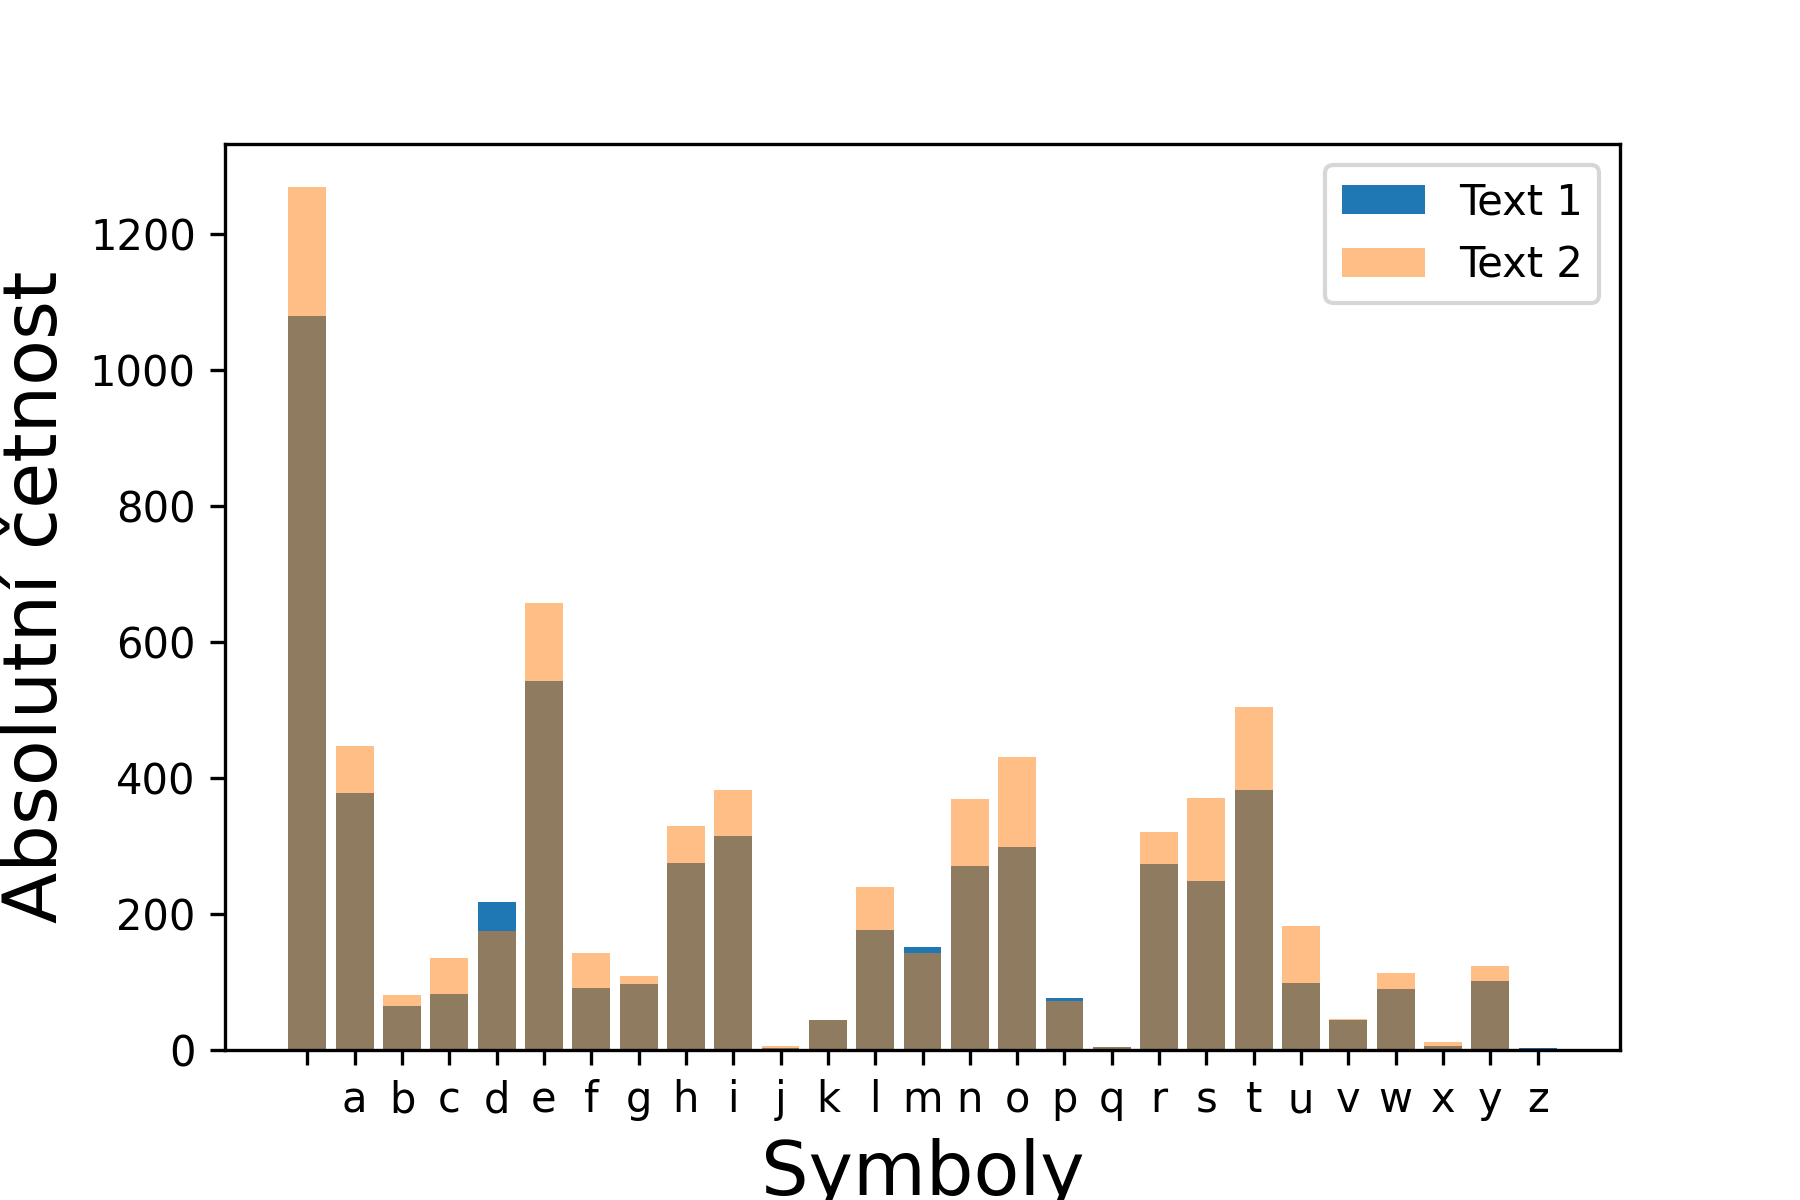
\includegraphics[width=\columnwidth]{img/abschdistr.png}
\caption{Graf absolutních četností symbolů obou textů.}
\label{fig:absch}
\end{figure}

\section{Úloha č.1}
\textit{Za předpokladu výše odhadněte matici přechodu Markovského řetězce pro \textbf{první} text. Odhadnuté pravděpodobnosti přechodu vhodně graficky znázorněte, např. použitím heatmapy.}\\

Dle předpokladu je první text vygenerován z homogenního Markovského řetězce s diskrétním časem. Tedy $ i $-tý symbol textu je stav Markovského procesu v čase $ i - 1 $. Dvojice sousedních symbolů znázorňují přechody tohoto procesu.

Maximálně věrohodným odhadem matice přechodu Markovského procesu je matice s prvky \\ $ {\hat{\textbf{p}}_{ij} =\frac{n_{ij}}{n_{i\bullet}}} $, tedy matici přechodu jsem odhadli pomocí četností přechodů. Výslednou matici přechodu $ \hat{\textbf{p}} $ jsme graficky znázornili pomocí zmíněné heatmapy, kterou lze pozorovat na obrázku \ref{fig:heat}. Matice má rozměry 27 $ \times $ 27. 26 za písmena anglické abecedy a 1 za symbol mezery.

\begin{figure*}[!ht]
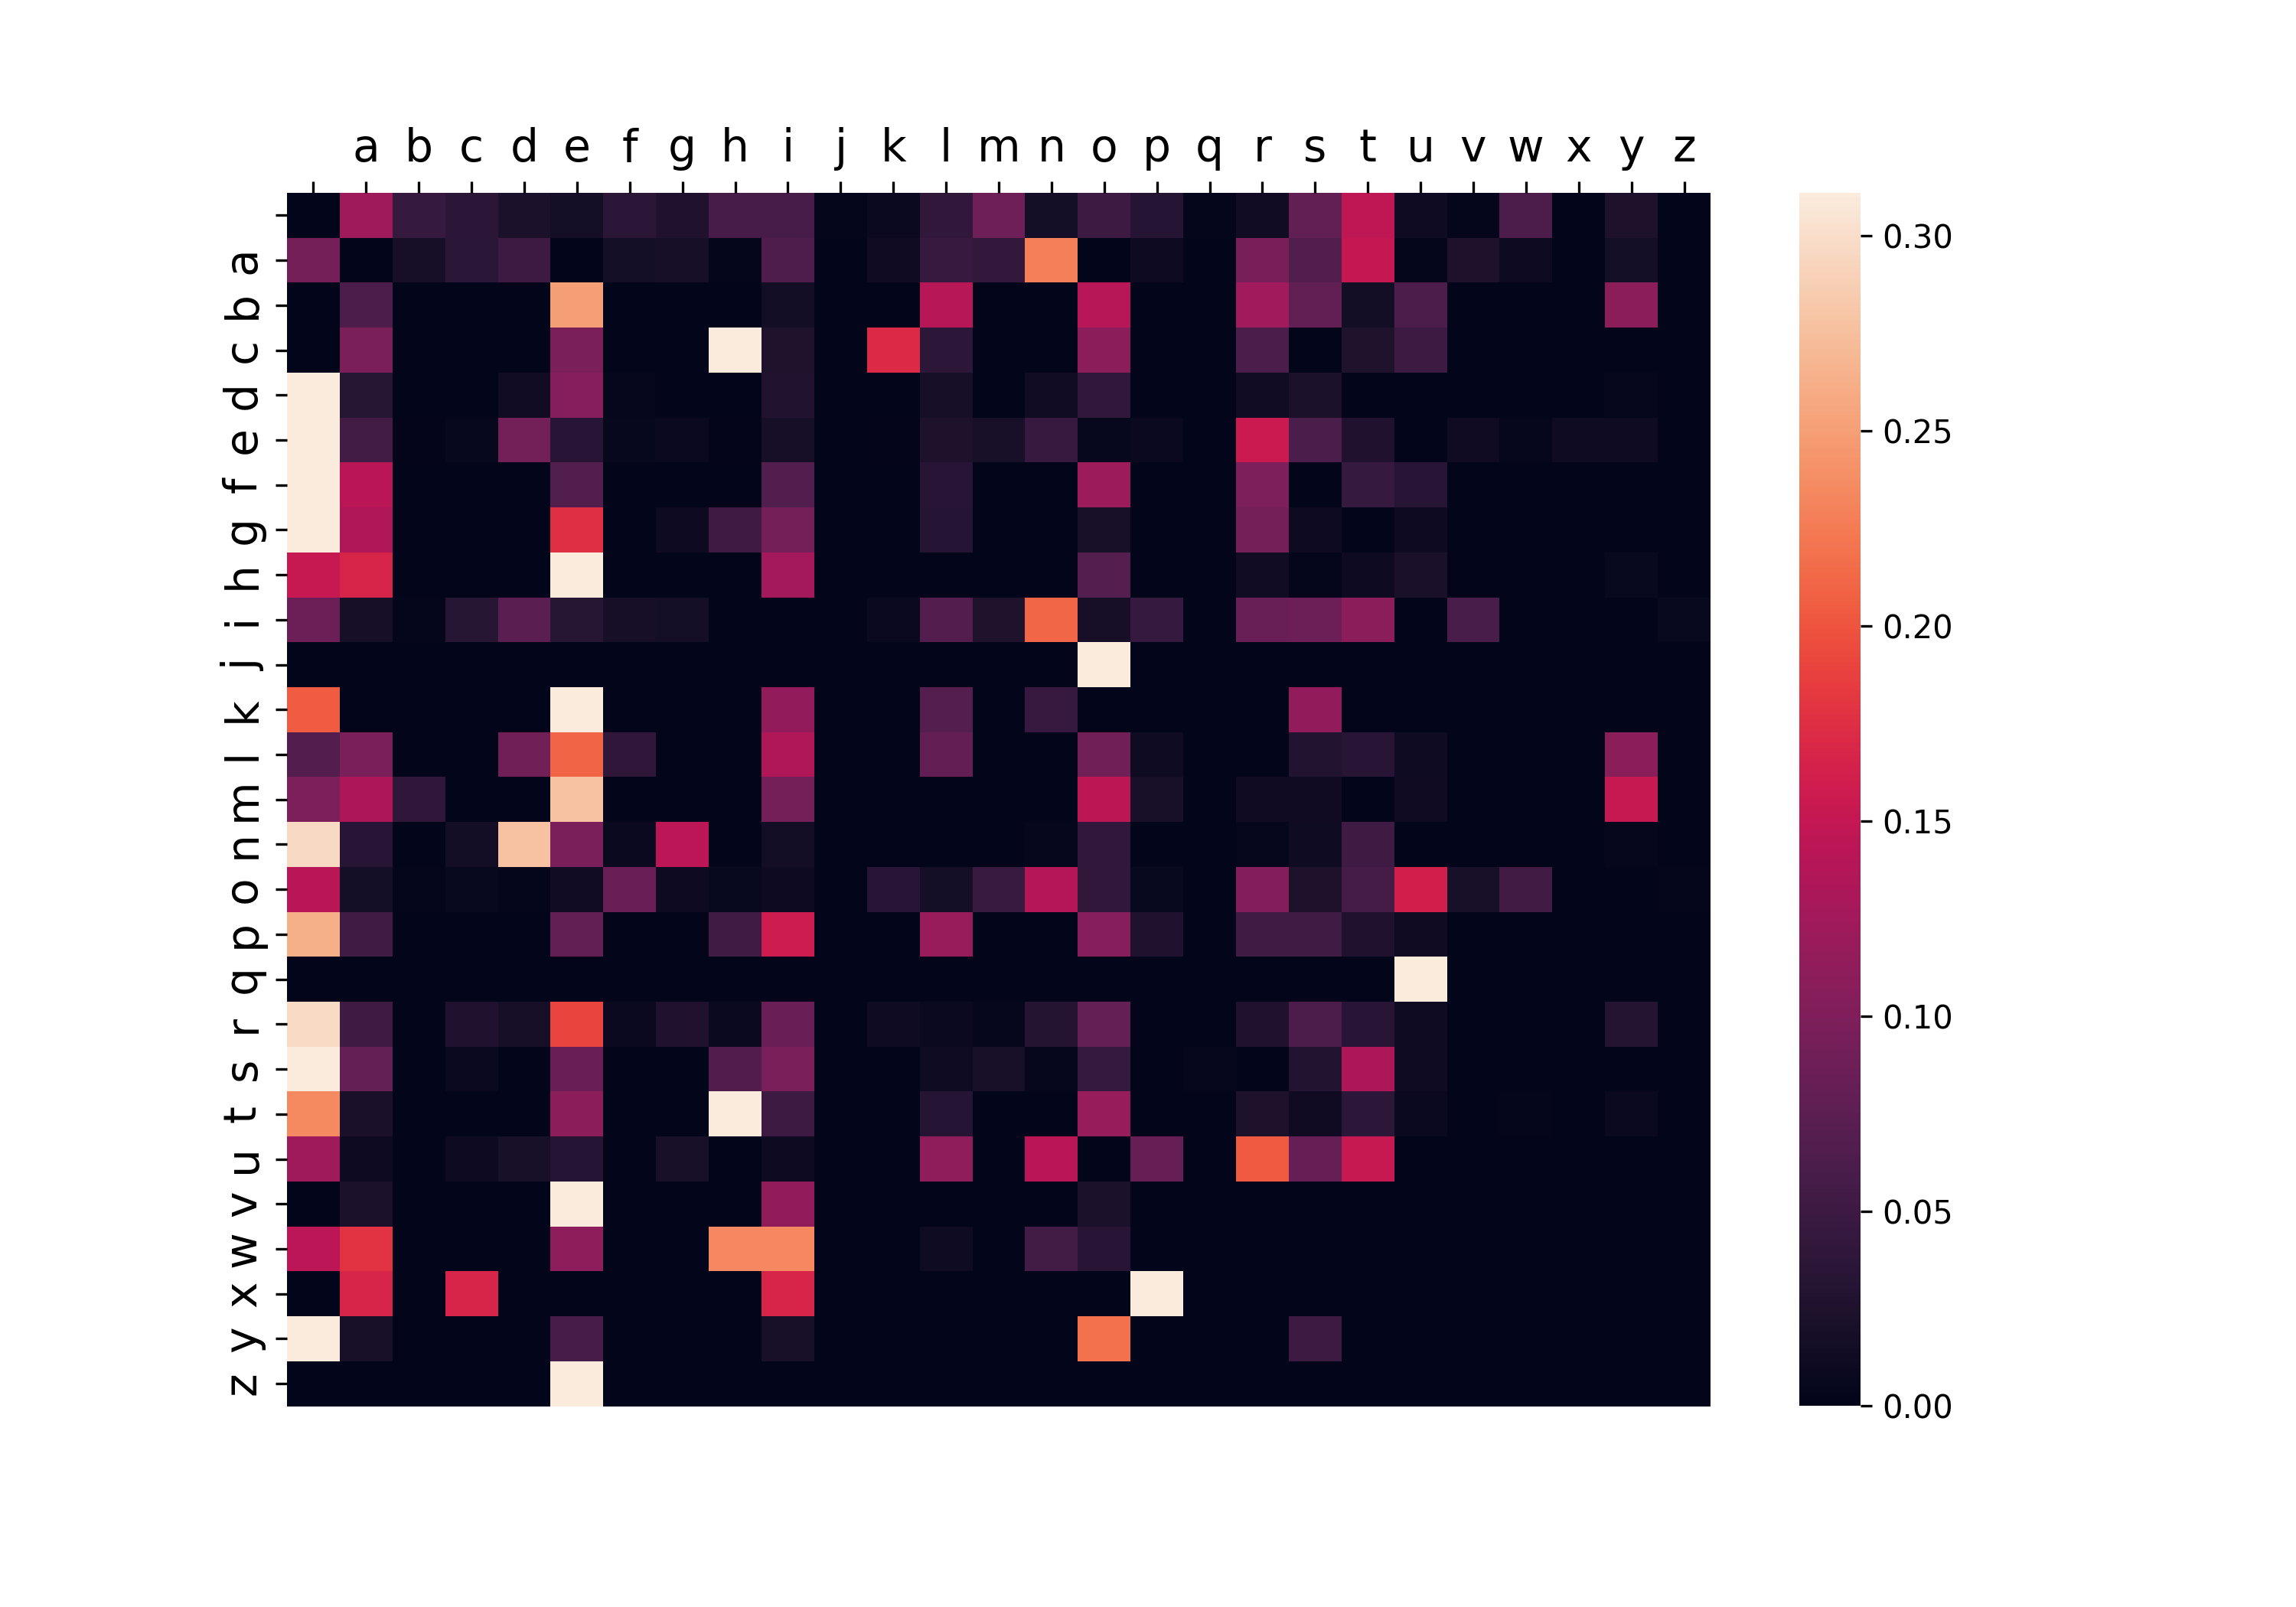
\includegraphics[width=\textwidth]{img/heatmapp.png}
\caption{Heatmapa odhadu matice přechodu homogenního Markovského řetězce prvního textu.}
\label{fig:heat} 
\end{figure*}

\section{Úloha č.2}
\textit{Na základě matice z předchozího bodu najděte stacionární rozdělení $ \bm{\pi} $ tohoto řetězce pro \textbf{první} text.}\\

Dle typu Markovského procesu, tedy generace textu, jsme odhadli, že množina stavů je již nerozložitelná, tj. všechny dvojice symbolů jsou navzájem dosažitelné. Toto platí pro všechny stavy, tedy celý Markovský řetězec nazýváme nerozložitelný. Dále víme, že v řetězcích s konečným počtem stavů neexistují stavy trvalé nulové. Tedy platí, že všechny stavy v našem zkoumaném Markovském řetězci jsou trvalé nenulové. Také tvrdíme, že jsou aperiodické.

Na základě předchozích vlastností a tvrzení můžeme využít větu o existenci stacionárního rozdělení a konkrétně její druhý bod, který říká: \\
\textit{Jsou-li všechny stavy trvalé nenulové, stacionární rozdělení $ \bm{\pi} $ existuje a je jediné.}\\
\textit{Jsou-li navíc všechny stavy aperiodické, platí}
\begin{equation*}
\bm{\pi} = \lim_{n \to +\infty} \bm{p}(n) \textrm{ pro libovolné } \bm{p}(0).
\end{equation*}
Na základě vlastností homogenního Markovského řetězce a vícekrokových pravděpodobností přechodu platí rovnost $ \bm{p}(n) = \bm{p}(0) \cdot \textbf{P}^n $. Tedy pro libovolné $ \bm{p}(0) $, splňující podmínky stacionárního rozdělení, získáme rozdělení $ \bm{\pi} $ následovně $ \bm{\pi} = \bm{p}(0) \cdot \textbf{P}^n $. Limitně pro $ n \to +\infty $ obsahuje matice $ \textbf{P}^n $ požadované rozdělení $ \bm{\pi} $ ve svých řádcích. Numericky je toto iterativní metoda, tedy provádíme výpočet do té doby, dokud nedosáhneme požadované přesnosti. Pro $ n = 10000 $ jsme dostali rozdělení, pro které platí $ \|\bm{\pi}\textbf{P}-\bm{\pi}\| < 10^{-15} $.

Druhou metodou je využití lineární algebry, vlastností vlastních čísel a vlastních vektorů. $ \bm{\pi}\textbf{P}=\bm{\pi} /^T $ po transponování celé rovnice dostáváme $ \textbf{P}^T \bm{\pi}^T = \bm{\pi}^T $, což je velice podobné rovnici vlastních čísel $ \textbf{A}\bm{x} = \lambda \bm{x} $, kde $ \lambda = 1 $. Tedy hledaným rozdělením $ \bm{\pi} $ je vlastní vektor vlastního čísla rovného(nebo velice blízkého) 1, přeškálovaný, aby platily podmínky $ \Sigma_{i \in S} \bm{\pi}_i = 1 $ a $ \forall i \in S: \bm{\pi}_i \geq 0 $. Takto získané rozdělení mělo normu od nulového vektoru srovnatelně malou jako rozdělení získané iterativní metodou, tedy $ \|\bm{\pi}\textbf{P}-\bm{\pi}\| < 10^{-15} $.

\section{Úloha č.3}
\textit{Porovnejte rozdělení znaků  \textbf{druhého} textu se stacionárním rozdělením $ \bm{\pi} $, tj. na hladině významnosti 5\% otestujte hypotézu, že rozdělení znaků \textbf{druhého} testu se rovná rozdělení $ \bm{\pi} $ z předchozího bodu.}\\

\begin{figure}[!h]
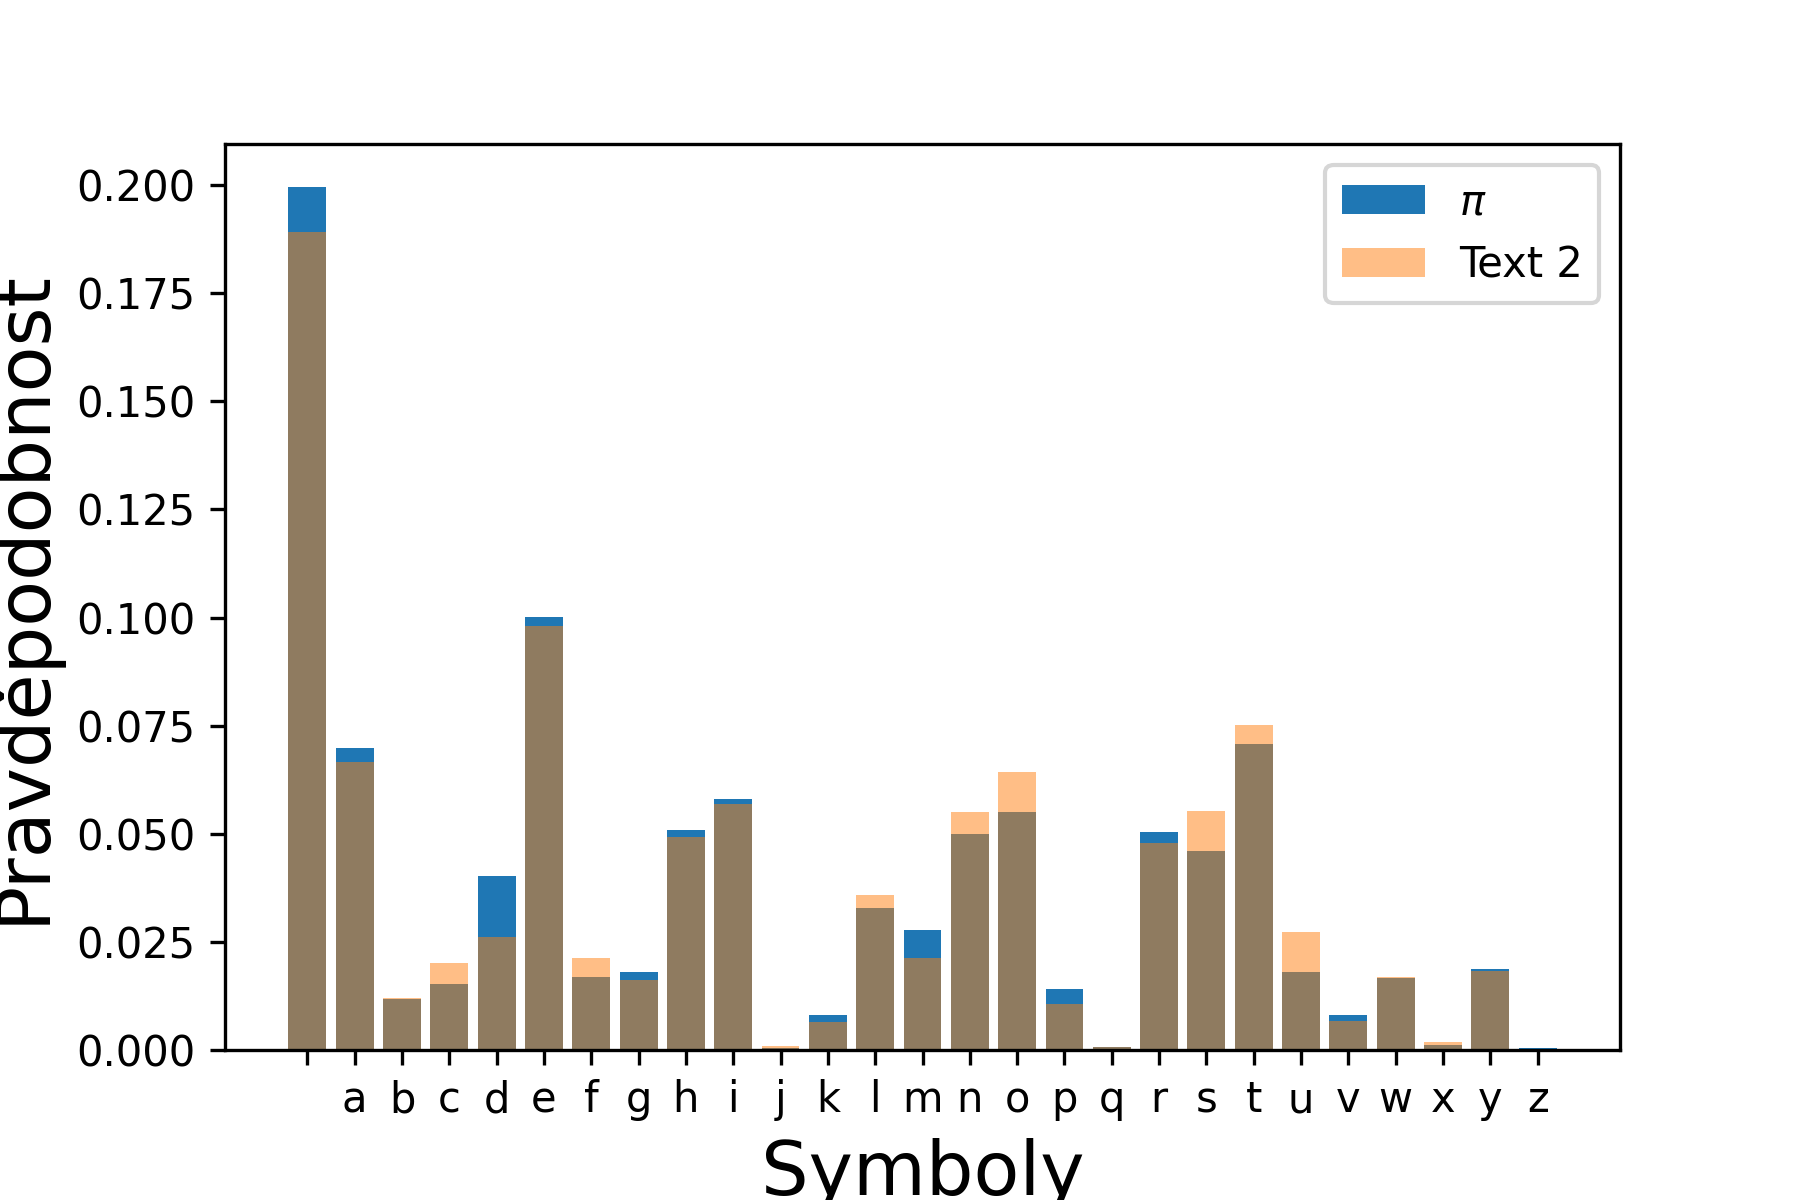
\includegraphics[width=\columnwidth]{img/pit2distr.png}
\caption{Graf stacionárního rozdělení $ \bm{\pi} $ a relativních četností symbolů druhého textu.}
\label{fig:pitd}
\end{figure}

Stacionární rozdělení $ \bm{\pi} $ a rozdělení znaků druhého textu lze pozorovat na obrázku \ref{fig:pitd}. Úlohou bylo otestovat, zda se tato dvě diskrétní multinomická rozdělení rovnají. K tomuto jsme využili test dobré shody, v tomto případě se známými parametry. Za nulovou hypotézu jsme postavili rovnost pravděpodobností $ H_0: \bm{p}=\bm{\pi} $, alternativní hypotézou byla nerovnost $ H_A: \bm{p}\neq \bm{\pi} $. Testovou statistikou byla $ \chi^2 $ statistika. Knihovna SciPy nabízí funkci \textit{chisquare}, která na vstupu bere naměřené a teoretické četnosti a vrátí testovou statistiku společně s p-hodnotou. Jelikož data nesplňují všude podmínku teoretických četností $ np_i \geq 5 $, tak jsme si testovou statistiku naprogramovali sami, a pro každý symbol jsme pozorovali, jak tyto četnosti přispívají do výsledné hodnoty. Největšími nárůsty byly symboly \textit{d} a \textit{u}, které teoretické četnosti splňovaly, samy zvýšily hodnotu $ \chi^2 $ o 64.6, což stačí k překročení kritické hodnoty, tedy na základě tohoto pozorování považujeme výsledek za správný i přes nedostatek dat. Dle p-hodnoty zamítáme nulovou hypotézu $ H_0 $ ve prospěch alternativní hypotézy $ H_A $, což je silným výsledkem a s velikou pravděpodobností můžeme věřit tomu, že se tato rozdělení nerovnají.

\begin{align*}
\chi^2 &= 145.2\\
\hat{p} &= 1.5 \cdot 10^{-18}\\
\chi^2_{0.05,26} &= 38.8
\end{align*}

\end{document}